This chapter summarizes previous efforts in numerical simulations of prismatic HTGRs.
The simulation of prismatic HTGRs require the coupled modeling of the neutronics and thermal-fluid phenomena.
This chapter comprehends the following sections: Section \ref{sec:litreview-neut} addresses diffusion methods for solving the neutronics, Section \ref{sec:litrev-thermalf} focuses on the thermal-fluids, Section \ref{sec:litreview-multi} studies the coupled simulations, and Section \ref{sec:litreview-summary} wrapps up the main takeaways of the literature review.

\section{Prismatic HTGR Diffusion Solvers}
\label{sec:litreview-neut}

Currently, several software programs solve the neutronics of prismatic \glspl{HTGR}.
Most of these codes rely on one of the following methods: stochastic transport (Monte Carlo), deterministic transport, or deterministic diffusion.
This section focuses on the last class.
% If time permits work on a brief description of the Monte Carlo and deterministic transport maybe.
% Why? Deterministic diffusion solvers have lower computational requirements than other methods reference ??
% The utilization of the Monte Carlo codes is unattractive because of the tremendous problem size and the need for a large number of neutron histories \cite{lee_status_2006}.
% It is one of the simplest means to solve neutron transport problems \cite{leppanen_development_2007}.
% Here I say the following
% Deterministic diffusion methods are computationally cheaper than the other methods.
% This characteristic makes it a good candidate for coupled calculations.

The history of deterministic diffusion solvers began in the late 1950s with the \gls{FDM} application to the analysis of \glspl{LWR}.
In \gls{FDM}, mesh spacings are usually of the order of the diffusion length.
While solving large multi-dimensional problems, this feature causes the mesh points to reach intractable numbers \cite{lewis_finite_1986}.
The computational expense of these calculations motivated the generation of more computationally efficient techniques \cite{lawrence_progress_1986}.
Although substantial overlaps exist, the most common techniques fall into two broad categories: nodal methods and \gls{FEM}.

% NODAL
FLARE \cite{delp_flare_1964} is a three-dimensional \gls{BWR} simulator, and it is representative of the first generation of nodal methods.
This approach used adjusted parameters to match actual operating data or the results of more accurate calculations.
Most of these methods were implementations of the so-called "1.5 group theory" \cite{gupta_nodal_1981}.
The second generation of nodal methods derived spatial coupling relationships by applying the \gls{TIP}.
This procedure obtains equivalent one-dimensional equations by integrating the multi-dimensional diffusion equation over directions transverse to each coordinate axis \cite{lawrence_progress_1986}.
This approach proved to be highly efficient and accurate in Cartesian geometries.

In 1981, a formulation based on the \gls{NEM} first demonstrated the feasibility of nodal methods in hexagonal geometries \cite{duracz_nodal_1981}.
However, this method would introduce non-physical singular terms that required the utilization of discontinuous polynomials.
This drawback motivated the development of more effective formulations.
HEXNOD, introduced in 1988 by Wagner \cite{wagner_three-dimensional_1989}, is an example of such formulations.
This algorithm uses the \gls{TIP} and, in contrast to the \gls{NEM}, solves the resulting differential equation analytically.
Wagner's article demonstrated the method's good accuracy by comparing to \gls{FDM} and Monte Carlo calculations for a few benchmark problems.

HEXPEDITE \cite{fitzpatrick_hexpedite_1992} introduced a new method that is another example of more effective formulations.
HEXPEDITE uses the \gls{TIP} formulation to derive a pseudo-one-dimensional equation.
The resulting differential equation is solved analytically.
The difference from HEXNOD is that HEXPEDITE uses a simpler and more efficient coupling scheme.
Different works \cite{fitzpatrick_hexpedite_1992}\cite{fitzpatrick_developments_1995} on the HEXPEDITE methodology tested the approach against the \gls{NEM} and the \gls{FDM}.
These studies established HEXPEDITE’s superiority in terms of accuracy and runtime.
HEXPEDITE's use prevailed in the analysis of \glspl{HTGR} until recently.
In 2010, \gls{INL} conducted a study \cite{ortensi_deterministic_2010-1} in which they compared HEXPEDITE's results against several diffusion codes, as well as the Monte Carlo codes MCNP5 \cite{rsicc_computer_code_collection_mcnp5_2003} and Serpent \cite{leppanen_serpent_2015}.
% In 2010, \gls{INL} conducted a study \cite{ortensi_deterministic_2010-1} in which they compared HEXPEDITE's results against the diffusion codes JAR, CITATION, and CRONOS2, as well as the Monte Carlo codes MCNP5 and Serpent.

DIF3D \cite{lawrence_dif3d_1983} and PARCS \cite{downar_parcs_2004} are other examples of prevalent nodal diffusion codes.
DIF3D has several solution options such as the diffusion \gls{FDM}, diffusion \gls{NEM} based on \gls{TIP}, and the VARIANT nodal transport method.
% VARIANT: variational nodal \cite{palmiotti_variant_1995}
PARCS has several solution options as well, such as a diffusion \gls{FDM}, diffusion \gls{NEM} based on \gls{TIP}, P$_{N}$ transport methods, and the multigroup transport simplified P$_3$ with \gls{FDM} and \gls{NEM} discretizations.

% from ortensi_deterministic_2010-1 and wang_modified_2018
Nodal methods solve relatively coarse meshes for approximate solutions.
This characteristic makes the process efficient.
On the other hand, the method does not provide detailed point-wise accurate solutions \cite{kang_finite_1973}.
Additionally, the derivation of nodal methods happens in a specific coordinate system for a particular node shape.
The application to complex problems is not flexible as different geometries require customized configurations.
This lack of flexibility limits the applications of nodal methods to regular geometries only.

% FEM
The \gls{FEM} is a well-established method in applied mathematics and engineering.
\gls{FEM} is a numerical technique for finding approximate solutions to partial differential equations by deriving their weak or variational form.
Most applications make \gls{FEM} preferable due to its flexibility in the treatment of curved or irregular geometries.
Also, the use of high order elements attains higher rates of convergence \cite{cavdar_finite_2004}.
The first engineering application of \gls{FEM} was in the field of structural engineering dating back to 1956.
In successive years, \gls{FEM} became the most extensively used technique in almost every branch of engineering.
\glspl{FEM} have several advantages over the nodal methods.
It provides flexibility in the geometry definition, a firm mathematical basis, ease in extension to the multi-group application, and high computational efficiency \cite{lee_development_2008}.

In 1973, Kang et al. \cite{kang_finite_1973} described the first application of \gls{FEM} to neutron diffusion theory.
The fundamental motivation for this development was the impractical application of the \gls{FDM} to three-dimensional problems.
In this early work, the author compared different \gls{FEM} approaches to the \gls{FDM} in one-dimensional and two-dimensional problems.
The studies showed a higher order of convergence achieved by the \gls{FEM}.

Throughout the last four decades, many software programs utilized the \gls{FEM} to solve the diffusion equation.
Some of the most recent software for diffusion simulations are CRONOS2 \cite{lautard_cronos_1990}, CAPP \cite{lee_development_2011}, and Rattlesnake \cite{wang_rattlesnake_2019}.
The list of \gls{FEM} diffusion solvers is more extensive, but we focus on the best-documented software in the open literature.
% We also emphasize that most of the \gls{FEM} diffusion solvers for \glspl{HTGR} were born as \gls{LWR} analysis codes.

% CRONOS
\gls{CEA} developed CRONOS2 \cite{lautard_cronos_1990} as part of the SAPHYR system.
It conducts steady-state and transient multi-group calculations, taking into account thermal-fluids feedback effects.
CRONOS2 solves either the diffusion equation or the transport equation using the S$_N$ method and an \gls{FDM} or a \gls{FEM} discretization.
In 2008, Damian et al. \cite{damian_vhtr_2008} conducted a study aimed at understanding the physical aspects of the annular core and the passive safety features of a standard block type \gls{HTGR}.
For the study, the authors developed the code suite NEPTHIS/CAST3M, which relied on CRONOS2.

% CAPP
In 2008, the \gls{KAERI} published an article \cite{lee_development_2008} that presented CAPP.
Its purposes are to conduct steady-state core physics analysis, core depletion analysis, and core transient analysis.
The article validated the code with two benchmark problems: the IAEA PWR benchmark problem, and Phase I Exercise 1 of the OECD/NEA PBMR-400 Benchmark \cite{reitsma_oecd-neansc_2008}.
The calculations of both problems changed the number of finite elements and the orders of shape functions.

In 2011, Lee et al. published an article \cite{lee_development_2011} in which they extended the functionalities of CAPP to prismatic \glspl{HTGR}.
To take into account the thermal feedback, the authors developed a simplified thermal-fluids analysis tool.
To validate their model, the authors simulated a two-dimensional model of the PMR-200 at the beginning of the equilibrium cycle.
The PMR-200 is a pre-conceptual reactor designed by \gls{KAERI}.
Their validation compared the results against HELIOS \cite{stammler_helios_1998}, concluding with a strong accuracy.
Moreover, the authors implemented a depletion solver based on the one-group flux determined by CAPP's diffusion solver.
The authors validated the depletion solver by calculating the multiplication factor as a burnup function of a single fuel block of the PMR-200.
They compared the results against HELIOS.
The maximum error was less than 200 pcm.

Tak et al. \cite{tak_cappgamma_2016} coupled CAPP and GAMMA+ \cite{lim_gamma_2006}.
GAMMA+ is a system code for thermal-fluids analysis and system transients.
They studied the steady-state performance of the PMR-200.
The authors conducted several studies, such as a core depletion calculation with and without a critical control rod position search and the analysis of the bypass flow effects on the coupled calculations.
Their results revealed that neglecting the bypass flow decreases the active core temperatures; consequently, the multiplication factor increases by approximately 300 pcm.
These results prove the importance of the right modeling of the thermal-fluids in prismatic HTGRs.

A recent article by Yuk et al. \cite{yuk_time-dependent_2020} added to CAPP the capability to conduct transient analyses.
This capability solves the time-dependent neutron diffusion equation with the \gls{FEM}.
The primary motivation behind this feature was to perform reactivity insertion accident simulations.
% Additionally, the article introduced a new method to resolve the control rod cusping effect \cite{joo_resolution_1984}.
% The new method integrates over partially rodded computation nodes, and the article referred to it as iPRN.
% To test its accuracy, the authors conducted two exercises with several techniques that reduce the rod cusping effect.
% The authors used the mesh reconstruction method to obtain the reference results, as such a method eliminates the rod cusping effect by updating the mesh at every time step.
% The iPRN technique showed higher accuracy than the other methods.
To test the new transient capabilities, they analyzed two control rod ejection scenarios and compared the results to those of the CAPP/GAMMA+ coupled code.
Both showed similar results.
This article highlights the importance of developing transient analysis capabilities to conduct accident simulations.

% Proghorn and Rattlesnake
RattleSnake \cite{wang_rattlesnake_2019} is the MOOSE \cite{gaston_moose_2009} based application for simulating the transport equation.
\gls{INL} had initially developed Pronghorn \cite{strydom_inl_2013} to model \glspl{PBMR}.
The MOOSE neutronics kernel library Yak incorporated the neutron diffusion models initially in Pronghorn.
Currently, RattleSnake is the primary tool for solving the linearized Boltzmann neutron transport equation within MOOSE and relies heavily on Yak.
Various solvers are available under RattleSnake, including low-order multigroup diffusion, spherical harmonics transport, and discrete ordinates transport, all solved with the \gls{FEM}.
% Both RattleSnake and Pronghorn yielded the same exact results when using the continuous \gls{FEM} multigroup diffusion option in RattleSnake.

% j_ortensi_relap-7_2012 j_ortensi_initial_2012
In 2012, \gls{INL} published a study \cite{j_ortensi_initial_2012} that coupled Pronghorn and RELAP-7 \cite{andrs_relap-7_2012}.
Pronghorn solved the coupled equations defining the neutron diffusion, fluid flow, and heat transfer in a three-dimensional model.
RELAP-7 is a MOOSE-based system application and solves the one-dimensional continuity, momentum, and energy equations for a compressible fluid.
It was responsible for simulating the plant system layout, including the hot and cold ducts, the helium circulator, and the steam generator.
% This study integrated PRONGHORN and RELAP-7 with the operator split approach (or loose coupling) where each application used an independent mesh.
To test the coupling, INL's team carried out the OECD/NEA MHTGR-350 Benchmark \cite{oecd_nea_coupled_2020}.
The original benchmark provides a set of 26 neutron energy group and temperature dependent cross sections.
To simplify the debugging, the authors collapsed the 26 groups into two groups.
Although using two groups reduces the accuracy of the model, the lower number of groups decreases the calculation time by at least a factor of ten.
In this study, a two-dimensional cylindrical model replaced the three-dimensional geometry defined by the benchmark.
The integrated system testing included two stages: (1) both stand-alone codes underwent several convergence studies, and (2) the integrated system solved the steady-state problem in an integrated manner.
The authors concluded that the coupling between Pronghorn and RELAP-7 was successful.

% strydom_inl_2013
In 2013, \gls{INL} conducted the OECD/NEA MHTGR-350 Benchmark \cite{strydom_inl_2013} without further simplifications.
The \gls{INL} team solved Phase I Exercise 1 using INSTANT-P1 \cite{wang_krylov_2011}, Pronghorn, and RattleSnake.
% They also solved exercises 2 and 3 using RELAP5-3D and PHISICS/RELAP5-3D code suit.
INSTANT-P1 is a transport solver that relies on the spherical harmonics discretization of angles.
The results for Pronghorn and RattleSnake were identical.
By modifying the cross-sections, INSTANT-P1 returned the diffusion solution.
Its results were within 30 pcm from Pronghorn and RattleSnake results.
All presented results exhibited good agreement with the benchmark results.

\subsection{Energy group structure analysis}

% Number of energy groups impact over the calculations
Diffusion calculations use homogenized group constants previously generated by neutron transport solvers.
The choice of the energy group structure for the group constant homogenization affects the accuracy of the diffusion calculation.
The longer neutron mean free path in \glspl{HTGR} compared to \gls{LWR} increases the spectral interactions between elements.
For this reason, HTGR analyses require more energy groups than conventional \gls{LWR} analyses.
This section summarizes previous studies on the impact of the energy group structure over the diffusion calculations.

\gls{ANL} directed a study \cite{lee_status_2006} to compare the accuracy of nodal diffusion calculations employing different energy group structures.
The group constant homogenization used the DRAGON neutron transport solver and the diffusion calculations utilized the code DIF3D.
For the study, the ANL team implemented a one-dimensional fuel-reflector model in which they compared the solution accuracy using 4, 7, 8, 14, and 23 energy groups.
They also used alternative energy group structures for the same number of groups.
For simplicity, the authors used the homogenized fuel compact model and generated all the group constant at 300 K.
One of their conclusions was that the number of energy groups should be more than 4, and more than 6 would be sufficient for uranium fueled HTGRs.
Another finding was that the accuracy of the diffusion calculation is sensitive to the energy group boundaries.
% Mention something about the metrics of the study? To asses the accuracy, they compared the multiplication factor.

% \begin{figure}[htbp!]
% 	\centering
% 	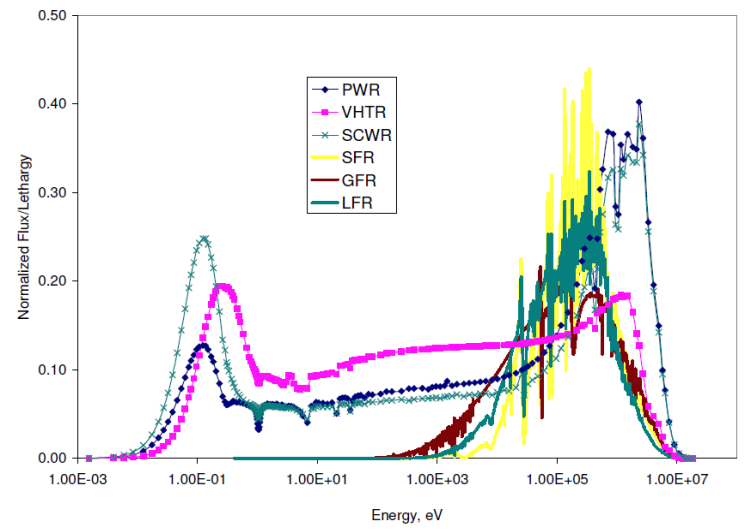
\includegraphics[width=0.40\linewidth]{figures/spectrum}
% 	\caption{Comparison of neutron energy spectra of different reactor designs. PWR=Pressurized Water Reactor, VHTR=Very High-Temperature Gas-Cooled Reactor, SCWR=Supercritical Water Reactor, SFR=Sodium Fast Reactor, GFR=Gas Fast Reactor, LFR=Lead Fast Reactor. Image reproduced from \cite{taiwo_summary_2005}.}
% 	\label{fig:spectrum}
% \end{figure}

% han_sensitivity_2008
Han's MS thesis \cite{han_sensitivity_2008} focused on selecting energy groups for the reactor analysis of the \gls{PBMR}.
The author used COMBINE6 \cite{grimesey_combinepc-portable_1994} for group constant generation and the Penn State nodal diffusion code NEM \cite{bandini_three-dimensional_1990} for the reactor analysis.
The author compared the results against MCNP5 reference results.
To simplify the setup, the model used uniformly distributed isotopes in the fuel.
The study performed the calculations at 300 and 1000 K.
To arrive at an optimal group structure, the author compared many combinations of group structures using a trial and error strategy.
One conclusion of this work agrees with the previous bibliography \cite{gulf_oil_company_nuclear_1973} \cite{duderstadt_nuclear_1976} in that the energy spectrum is critical to yield an accurate description of a nuclear reactor using a few groups.

ANL's study helps set up proper nodal diffusion calculations for an \gls{HTGR}.
Although we can extrapolate those conclusions to \gls{FEM} diffusion solvers, such a study might be valuable as a part of this thesis.
ANL's team conducted the study at 300 K --- not in the operational range of any \glspl{HTGR}.
On the contrary, Han's thesis included an analysis at 1000 K, and his results showed that the temperature changes have a non-negligible impact.
Additionally, ANL's study used the simplified model of the homogenized fuel compact.
Han highlighted that homogenized fuel models of the \gls{PBMR} underestimate criticality calculations.
In 2015, \gls{INL} presented their results \cite{strydom_results_2015} for an \gls{IAEA} \gls{CRP} \cite{tyobeka_htgr_2011} and showed that the homogenization of the compact material notably underestimates the multiplication factor.
On the other hand, the open literature has not investigated the impact of such simplification over the homogenized group constants.

\section{Prismatic HTGR Thermal-fluids}
\label{sec:litrev-thermalf}

% sort of motivation
Thermal-fluids calculations enable the correct design of \glspl{HTGR}.
Predicting the maximum fuel temperature at steady-state is of paramount importance to succeed in such a task.
We emphasize this statement in the case that hydrogen production is desirable, as that process requires higher coolant temperatures, leading to high fuel and reactor vessel temperatures.

% sort of intro to simplified models
The complex geometry of the hexagonal fuel assembly requires numerical calculations for obtaining accurate evaluations.
Thermal-fluids studies for early \glspl{HTGR} consisted mainly of support calculations for \gls{NRC} safety analysis reports.
The analyses employed sets of independent solvers that relied on simplified approximations.
Simplified models help understand some fundamental aspects of prismatic \glspl{HTGR} and have the advantage of reducing the computational expense of the calculations.

% shenoy_htgr_1974
General Atomics \cite{shenoy_htgr_1974} developed the first set of software libraries that relied on simplified approximations.
The following list introduces and summarizes some of these and their features:

\begin{itemize}
\item FLAC: It determines the coolant flow distribution in the coolant channels and gaps.
It solves the one-dimensional momentum equation for incompressible flow and the continuity equations for mass and energy.

\item POKE: It determines the coolant mass flow, coolant temperature, and fuel temperature distribution.
It solves the steady-state mass and momentum conservation equations for parallel channels.

\item DEMISE: It determines the steady-state three-dimensional temperature distribution in a standard element.
It solves the temperature in a network model.

\item TAC2D: It is a general-purpose thermal analysis code.
It solves the two-dimensional heat conduction equation.
\end{itemize}

Several studies have used these software programs.
% macdonald_ngnp_2003
For example, \gls{INL} conducted in 2003 a design study \cite{macdonald_ngnp_2003} in support of the \gls{NGNP} project.
It aimed to investigate options for the NGNP that increase the coolant temperature with the lowest possible inlet temperature and the highest overall core power.
The authors conducted several parametric studies whose reference reactor was the GT-MHR \cite{general_atomics_gas_1996}.
Using POKE, they evaluated two major design modifications: reducing the bypass flow and better controlling the inlet coolant flow distribution.
Reducing the bypass flow fraction from 20$\%$ to 10$\%$ reduces the peak fuel temperatures by about 50$^{\circ}$C.
Controlling the inlet flow distribution has a stronger effect.
Other studies focused on the dimensions of the reactor and their impact on the maximum fuel temperature.
Using POKE and TAC2D, the authors investigated taller and higher power reactor cores.
The investigation included a 10-block-high 600 MWt, a 12-block-high 720 MWt, and 14-block-high 840 MWt.

Among the simplified approaches, this thesis differentiates the flow network, equivalent cylindrical model, and unit cell model.
% flow network model
% reza_design_2006
Using the network analysis tool RELAP5-3D/ATHENA \cite{inl_relap5-3dathena_2005}, Reza et al. \cite{reza_design_2006} conducted a thermal-fluids study of the GT-MHR.
Reza et al. increased the reactor outlet temperature to enable hydrogen production.
Additionally, they evaluated alternative coolant inlet flow configurations in an attempt to reduce the reactor vessel temperatures.
After finding an optimal configuration, they evaluated the fuel and the reactor vessel's maximum temperatures during the \gls{LPCC} and the \gls{HPCC} events.

% equivalent cylindrical model
% no_multi-component_2007
An example of an application using the equivalent cylindrical approach is GAMMA \cite{no_multi-component_2007}.
Its main objective is simulating the air ingress event following a LOCA.
Following the depressurization of helium in the core, air could potentially enter the core through the break and oxidize the in-core graphite structure.
Graphite oxidation is an exothermic chemical reaction and, thus, it is a significant concern.
GAMMA solves heat conduction, fluid flow, chemical reactions, and multi-component molecular diffusion.
The code couples the solid and gas equations using the porous media model.
Together with the multi-dimensional analysis feature, GAMMA has a one-dimensional analysis capability for  modeling a flow network.

% takada_core_2004
Takada et al. \cite{takada_core_2004} carried out another study using the flow network and the equivalent cylindrical model.
Focusing on the \gls{HTTR}, they developed a thermal-fluids design code.
This used the flow network analysis code FLOWNET \cite{maruyama_verification_1988} for calculating the coolant flow and temperature distributions.
TEMDIM \cite{maruyama_verification_1988} solved the fuel temperatures using the equivalent cylindrical model.
Finally, the authors validated the calculation scheme by comparing its results with the experimental data from the \gls{HTTR}.

% unit cell model
% nakano_conceptual_2008
Nakano et al. \cite{nakano_conceptual_2008} studied different fuel assembly configurations using several simplified approximations.
For determining the fuel temperature, they used TAC2D.
% A previous nuclear analysis calculated the power density.
A previous study calculated the flow distribution using FLOWNET.
The fuel temperature calculation used the equivalent cylindrical model for a hot channel unit cell.
However, the asymmetry of the unit cell configuration makes the temperature distribution asymmetric in the graphite block.
The equivalent cylindrical model fails to capture this behavior.

% in_three-dimensional_2006
In 2006, In et al. \cite{in_three-dimensional_2006} conducted a more detailed analysis using a three-dimensional model of the unit cell in the hot-spot of an \gls{HTGR}.
The objective of the study was to predict the maximum fuel temperature at steady-state.
The analysis focused on the GT-MHR 600 at the end of the equilibrium cycle.
The CFD code CFX 10 \cite{ansys_inc_cfx_2006} calculated the three-dimensional temperature profile.
The results showed that the maximum fuel temperature surpassed the design limits, so the authors proposed a countermeasure accordingly.

% more detailed calculations
Such simplified approaches are helpful to understand essential aspects of prismatic \glspl{HTGR} but they may affect the temperature distribution.
More detailed thermal-fluids evaluations were rare in the open literature until the last 15 years.

% cioni_3d_2005
Cioni et al. \cite{cioni_3d_2005} presented an article in 2005 in which they conducted three-dimensional simulations of fuel assemblies of an \gls{HTGR}.
The study's objective was to investigate an emergency situation due to the blocking of cooling channels in the core.
They used the \gls{CFD} code Trio\_U \cite{bieder_priceles_2000} to carry out the analysis.
The numerical scheme solved the three-dimensional conduction equation in the solid coupled to the coolant's one-dimensional thermal-fluid equations.
% In the preliminary work, the authors conducted a study of the bypass flow's influence on the maximum coolant and fuel temperature.
A preliminary study analyzed the consequences of two different blocking in a portion of a fuel assembly.
A central blockage exhibited a stronger influence over the assembly's maximum temperatures compared to a peripheral blockage.
Last, they investigated two configurations.
First, six fuel elements surrounded the fuel element with the blockage.
Second, five fuel elements and one reflector element surrounded the fuel element with the blockage.
The blockage increased the temperature on the blocked fuel assembly only and it did not affect the surrounding elements due to the bypass flow.
The results also show that the fuel temperature surpassed the design limits and that the reactor operators should counteract these effects with active systems.

% simoneau_three-dimensional_2007
Simoneau et al. \cite{simoneau_three-dimensional_2007} analyzed the transient behavior of an \gls{HTGR} during the \gls{DCC} and \gls{HPCC} event.
The CFD code STAR-CD \cite{computational_dynamics_limited_star-cd_2004} performed the calculations.
It solved conductive, convective, and radiation heat transfer in a 30$^{\circ}$ section of the core and reactor vessel.
It used the porous media model to accommodate the different spatial scales.
The model did not resolve the boundary layer, and the use of coefficients prescribed the solid-fluid heat transfer and pressure drop across the core.
The authors validated their model against explicit calculations using a single fuel block.
One of their results showed that the maximum temperature in the \gls{HPCC} event is lower than in the \gls{DCC} event.
However, the extra convective heat transfer caused a thermal stratification in the surrounding air, causing higher temperatures in the upper reactor structures.

% tak_numerical_2008
In 2008, an article by Tak et al. \cite{tak_numerical_2008} conducted  a three-dimensional \gls{CFD} analysis on a typical prismatic \gls{HTGR} fuel column.
The commercial code CFX 11 \cite{ansys_incorporated_cfx_2006} performed the calculations.
The fuel column under study was from the PMR-600, a pre-conceptual reactor designed by \gls{KAERI} whose reference design is the GT-MHR.
The study considered a one-twelfth section of the fuel due to its symmetry.
The model determined the coolant distribution using the one-dimensional thermal-fluid equations.
Such coolant distribution served as input to the CFD code.
The friction in the channels is dependent on the viscosity, which is highly dependent on the temperature.
Therefore, obtaining the mass flow rates from a separate solver may introduce errors \cite{sato_computational_2010}.
As mentioned earlier, the unit cell model may introduce errors in the maximum temperature prediction.
To assess the accuracy of the unit cell model, the authors compared the CFD results against the unit cell model results.
The unit cell model does not consider the bypass flow between assemblies or the radial power distribution within the fuel assembly.
Tak et al. conducted a parametric study that analyzed the bypass gap size's impact on the maximum fuel temperature.
By increasing the bypass gap, the maximum fuel temperature grows.
The results of this study indicate that the accuracy of the unit cell worsens for larger gaps.
Another study imposed different radial peaking factors for the different fuel channels.
Such a study showed the effects of considering a non-flat radial power distribution.
The authors considered a radial power distribution that did not strongly impact on the maximum fuel temperature.

% left here in the review

% sato_computational_2010
Another article \cite{sato_computational_2010} carried out \gls{CFD} calculations of a typical prismatic \gls{HTGR} with the commercial code FLUENT \cite{fluent_inc_fluent_2006}.
Their modeled a one-twelfth section of the fuel column of the GT-MHR.
The authors conducted parametric studies changing several factors, such as bypass gap-width, turbulence model, axial heat generation profile, and geometry changes due to irradiation.
Their most relevant results show that the bypass flow causes a large lateral temperature gradient in the block.
Large temperature gradients cause excessive thermal stresses, which raise potential structural issues.
The authors compared the results from different turbulence models: $k \sim \varepsilon$ and $k \sim \omega$.
The $k \sim \omega$ model predicted bulk temperatures that are considerably lower than those from the $k \sim \varepsilon$ model.
The maximum temperature difference was 49$^{\circ}$C.
The overall mass flow rate was about 10$\%$ greater for the $k \sim \omega$ model.
The study suggested that these turbulence models need more verification against prismatic \gls{HTGR} experiments.
Another study analyzed the effect of considering different peak radial factors.
This consideration introduced variations of the maximum fuel temperature of up to 160 $^{\circ}$C.
Their last study focused on the effects of the graphite dimensional changes on the temperature profile.
The shrunken column showed considerably lower temperatures in the fuel.

% travis_thermalhydraulics_2013
Despite the recent developments in CFD tools, a detailed full-core analysis for a prismatic \gls{HTGR} still requires a tremendous computational expense.
This requirement is mostly due to the three-dimensional CFD simulation of the coolant flow.
Travis et al. \cite{travis_thermalhydraulics_2013} developed a method to compute full-core thermal-fluids analyses of \glspl{HTGR}.
The article presented a simplified method that reduces the computational time and memory requirements while maintaining accurate results.
The method solves the three-dimensional heat conduction in the solid and the one-dimensional thermal-fluid equations in the channels.
The fluid one-dimensional approximation avoids finer meshes near the walls as well as turbulence conservation equations \cite{tak_development_2014}.
The method's validation analyzed a fuel column and compared the results to those of a three-dimensional CFD simulation.
The CFD simulation used the commercial software STAR-CCM+ \cite{cd-adapco_star-ccm_2012}.
The new computational scheme reduced the computation time to 2.5\% of the CFD simulation time.
The new method provided good predictions of the temperature distribution and the axial variation of the helium bulk temperature.
However, it failed to resolve the velocity and temperature distribution within the boundary layer properly.
Overall, the method showed good accuracy and less than a 2\% difference to the CFD simulation.

% tak_practical_2012 / tak_development_2014
Tak et al. \cite{tak_practical_2012} \cite{tak_development_2014} developed CORONA, which uses a practical method for the whole core analysis.
CORONA intends to combine the accuracy from CFD tools and the light computational expense of system analysis codes.
The method solves the three-dimensional heat conduction equation in the solid and the one-dimensional thermal-fluid equations in the fluid.
To enhance practicability, the code adopts a basic unit cell concept, which eliminates an elaborate grid generation process.
The basic unit cell concept is an extension of the traditional unit cell method, which uses a single triangular unit cell.
This method considers various shapes of unit cells as well as the heat transfer between them.
The method provides a way for fast generating computational grids for modeling the solid regions.
To validate CORONA, the authors compared its results against CFX and experimental results.
The validation results showed that CORONA provided reasonably accurate results.

% end of section
CFD techniques allow the detailed temperature profile over local models to be computed.
The fine mesh requirement imposes high computational costs for a whole-core CFD analysis, restricting such methods.
However, a whole-core thermal analysis has many advantages over local models.
In general, the problem set up includes more accurate boundary conditions.
Without whole-core modeling, the local models' mass flow distributions are average values of the core flow rate instead of their exact value \cite{huning_novel_2016}.
This simplification leads to under-predicted fuel temperatures for the assemblies with a lower flow rate than the average.
Additionally, a coupled analysis with a reactor physics code requires a full-core model \cite{tak_practical_2012}.

% this might appear in a summary of the chapter: see travis_thermalhydraulics_2013 / tak_practical_2012 / tak_development_2014 
% The fine mesh requirement for a whole core CFD analysis restricts the use of such methods.
% Most of the CFD studies limit their application to the local behavior of a fuel column.
% The alternative for an explicit whole-core analysis are system codes that use simplified models.
% However, the simplification of the geometries reduces the fuel block temperature resolution.
% The present method intends to overcome the difficulties in CFD calculation as well as in system calculations.
% The computational expense of a solid heat conduction equation is much less than that of fluid conservation equations in CFD analyses .
% This requirement is mostly due to the three-dimensional CFD simulation of the coolant flow.
% The methodology provides good predictions of the global parameters such as the three-dimensional spatial temperature distribution and the axial variation of the helium bulk temperature \cite{travis_thermalhydraulics_2013}.
% The fluid one-dimensional approximation avoids finer meshes near the walls as well as turbulence conservation equations \cite{tak_development_2014}.

\section{Prismatic HTGR Multi-physics}
\label{sec:litreview-multi}

% sort of intro
Historically, stand-alone simulations have solved the neutronics and thermal-fluids of \glspl{HTGR}.
Nonetheless, these physical aspects describe processes that rely heavily on one another.
Hence, a coupled analysis is necessary to consider the interaction between the neutronics and thermal-fluids behavior \cite{tak_cappgamma_2016}.

% damian_vhtr_2008
In 2008, Damian et al. \cite{damian_vhtr_2008} conducted a study aimed to understand the physical aspects of the annular core and the passive safety features of a prismatic \gls{HTGR}.
They performed analyses on various geometrical scales, including: unit cell and fuel columns located at the core hot-spot and two-dimensional and three-dimensional core configurations, including the coupling between neutronics and thermal-fluids.
The first part of the assessment concerns thermal calculations on steady-state core configurations.
Such a study used CAST3M \cite{studer_cast3marcturus_2007} to solve the three-dimensional heat conduction in the solid coupled with the one-dimensional thermal-fluid equations in the coolant.
% The authors conducted a parametric study on the maximum fuel temperature by modifying the fuel compact and the fuel element geometries.
% An annular fuel compact and the reduction of the number of fuel compacts in the outer ring yielded the best performance.
The second part of the assessment used the transport code APOLLO2 \cite{sanchez_apollo2_1999} on a two-dimensional core configuration to minimize the radial power peaking factor.
The analyses included the variation of several parameters, such as fuel enrichment, fuel loading, and the fuel management scheme.
The fuel enrichment variation had the most substantial impact.
The last part of the study analyzed a three-dimensional core model using the coupled codes NEPTHIS \cite{cavalier_presentation_2005} and CAST3M/Arcturus.
NEPTHIS and CAST3M/Arcturus calculate the neutronics and the thermal-fluids, respectively.
NEPHTIS uses a transport-diffusion calculation scheme that relies on APOLLO2 and the diffusion code CRONOS2.
The CAST3M/Arcturus model uses a two-level approach.
On the first level, the porous media model solves the homogenized system and the coolant.
On the second level, CAST3M solves the thermal-fluids on the homogenized geometry.
The authors conducted several parametric studies and assessed their impact on the power distribution.
The studies included the variation of the helium bypass fraction, average power density, core geometry, reflector materials, and fuel loading strategy.
One of their results exhibited that with the reduction of the bypass fraction, the average reflector temperature rises.
Another result showed that using magnesium oxide as the reflector material yields lower temperatures for normal operation and transients.

% CAPP
In 2011, Lee et al. published an article \cite{lee_development_2011} in which they extended the functionalities of CAPP to prismatic \glspl{HTGR}.
To take into account the thermal feedback, the authors integrated into CAPP a simplified thermal-fluids tool.
This tool divides a fuel column into six triangular prisms.
Each of them hosts a representative coolant channel.
The code calculates the axial coolant temperature distribution solving the energy equation.
After calculating the coolant temperature, a two-dimensional conduction model solves the moderator and fuel compact temperatures.
Through a TRISO particle conduction model, the model obtains the fuel temperature.
Finally, a three-dimensional conduction model based on the \gls{FDM} allows for solving the reflector temperature.
% The cross-sections are a function of burnup, moderator temperature, and fuel temperature.
To validate this model, the authors solved a two-dimensional model of the PMR-200 at the beginning of the equilibrium cycle.
They compared the results against HELIOS reference results.
The results showed good accuracy.

% tak_coupled_2016
Tak et al. \cite{tak_coupled_2016} developed a neutronics/thermal-fluids coupled code using DeCART \cite{kaeri_decart_2007} and CORONA.
DeCART is a whole-core neutron transport code, and it was responsible for calculating the power distribution and the fast neutron fluence.
CORONA calculated the temperature distribution.
To validate the code, the authors conducted the OECD/NEA MHTGR-350 benchmark.
The exercise's main objective was to validate the code and identify technical challenges for future development.
The authors presented an interesting analysis in which they compared the coupled simulation results and the stand-alone simulations.
The difference in the multiplication factor was as high as 2597 pcm.
The axial offset and maximum fuel temperature exhibited significant differences as well.
Such a result highlights the importance of the integration of both neutronics and thermal-fluid solvers.

% tak_cappgamma_2016
Another article \cite{tak_cappgamma_2016} introduced a coupling between CAPP and GAMMA+.
GAMMA+'s primary motivation was to analyze the air ingress accident and thermo-fluid transients in \glspl{HTGR}.
It uses the one-dimensional form of the mass, momentum, energy, and species conservation equations to solve the fluid's flow and temperature distribution.
For solids, it uses three different models: (1) heat conduction model of a TRISO particle, (2) implicit coupling to consider the heat exchange between a fuel compact and TRISO particle, and (3) multi-dimensional heat conduction model of the hexagonal fuel and reflector blocks.
In such a study, the authors applied the coupled code to study the steady-state performance of the PMR-200.
They analyzed the bypass flow effects on the coupled calculations.
Some of their most relevant results showed that the maximum fuel temperature reaches a peak near the middle of the equilibrium cycle.
Another result revealed that neglecting the bypass flow decreases the active core temperatures and increases the reflector temperatures.
Consequently, the multiplication factor increased by approximately 300 pcm.
On the other hand, the power density changes were not appreciable.

% yuk_time-dependent_2020
A recent article by Yuk et al. \cite{yuk_time-dependent_2020} added the capability to conduct transient analyses to CAPP.
To take into account the thermal feedback, the authors developed a simplified thermal-fluids analysis tool.
The tool divides a fuel column into six triangular prisms.
Each of them hosts a representative coolant channel.
After calculating the coolant temperature, a two-dimensional conduction model solves the moderator and fuel compact temperatures.
CAPP code uses predetermined tables of thermal conductivity for each material.
For a given fast neutron fluence and temperature, it obtains the thermal conductivity by interpolation.
To test the new transient capabilities, they analyzed two control rod ejection scenarios.
They compared the results to those from the coupled CAPP/GAMMA+ code.
Both methods showed similar results.

% Benchmarks Intro
The prismatic \gls{HTGR} tools available have lagged behind state of the art compared to \glspl{LWR}.
This delay drives the development of more accurate and efficient tools to analyze the reactor behavior for design and safety evaluations.
In addition to the development of new methods, it is essential to define appropriate benchmarks to compare various tools' capabilities.
% oecd_nea_coupled_2020
In 2012, the \gls{OECD}/\gls{NEA} defined a benchmark for the \gls{MHTGR}-350 MW reactor \cite{oecd_nea_benchmark_2017}.
The purpose of this benchmarking exercise is to compare various coupled reactor physics and thermal-fluid analysis methods.
The MHTGR design serves as a basis for this benchmark.
The scope of the benchmark is twofold: (1) to establish a well-defined problem, based on a common given data set, to compare methods and tools in core simulation and thermal-fluid analysis, and (2) to test the depletion capabilities of various lattice physics codes available for prismatic \glspl{HTGR}.
The OECD/NEA MHTGR-350 MW benchmark subdivides the coupled system calculation into three phases.
Phase I corresponds to the stand-alone neutronics and thermal-fluids modeling, as well as the coupled neutronics/thermal-fluids steady-state modeling.
Phase II consists of transient cases.
Phase III focuses on lattice depletion calculations.

% tyobeka_htgr_2011 / strydom_results_2015
Sensitivity analysis and uncertainty analysis methods can assess the predictive capabilities of coupled neutronics/thermal-fluids simulations.
In 2013, the IAEA launched a \gls{CRP} \cite{tyobeka_htgr_2011} on the \gls{HTGR} Uncertainty Analysis in Modeling.
The \gls{CRP} objective was to determine the uncertainty in \gls{HTGR} calculations at all stages of coupled reactor physics/thermal-fluids and depletion calculations.
This \gls{CRP} is a natural continuation of the previous IAEA and OECD/NEA international activities \cite{iaea_evaluation_2003}\cite{reitsma_oecd-neansc_2008} on Verification and Validation of available \gls{HTGR} simulations capabilities.
The technical approach is to establish and utilize a benchmark for uncertainty analysis.
The benchmark defines a series of well-defined problems with complete sets of input specifications and reference experimental data.
The CRP adopted the MHTGR-350 as the reference design and the GT-MHR as a second reference design.
The design specification uses the OECD/NEA MHTGR-350 MW benchmark \cite{oecd_nea_benchmark_2017} code design specifications.
The CRP subdivides the coupled system calculation into three phases.
Phase I corresponds to the stand-alone neutronics and thermal-fluids modeling.
Phase II consists of design calculations, coupled with steady-state neutronics/thermal-fluids calculations with and without a depletion calculation.
Phase III focuses on safety calculations.

\section{Chapter Summary}
\label{sec:litreview-summary}

